\documentclass{article}
\usepackage{graphicx} % Required for inserting images
\usepackage{kotex}
\usepackage{listings}
\usepackage{xcolor}
\usepackage{hyperref}

\title{스택(Stack)}

\begin{document}

\definecolor{backcolour}{rgb}{0.95,0.95,0.92}
\definecolor{codegreen}{rgb}{0,0.6,0}
\definecolor{myred1}{rgb}{255, 0, 0}


% Define a custom style
\lstdefinestyle{myStyle}{
    backgroundcolor=\color{backcolour},   
    commentstyle=\color{codegreen},
    basicstyle=\ttfamily\footnotesize,
    breakatwhitespace=false,         
    breaklines=true,                 
    keepspaces=true,                 
    numbers=left,       
    numbersep=5pt,                  
    showspaces=false,                
    showstringspaces=false,
    showtabs=false,                  
    tabsize=2,
}

\hypersetup{
    colorlinks=true,
    linkcolor=blue,
    filecolor=magenta,      
    urlcolor=cyan,
}

\maketitle

\noindent 이론적 배경\\\\
먼저 이론적으로 스택이 무엇이고, 왜 배우는지 알아봅시다.\\\\
스택은 영어로 Stack이고, Stack은 쌓다라는 뜻이 존재합니다. 스택은 이름처럼 각 값을 블럭처럼 생각하여 순서대로 쌓아서 저장하고, 무너지지 않게 위에서 부터 꺼내여 활용하는 자료구조입니다. 재귀함수가 동작하는 과정에서 앞선 함수들의 변수 값을 저장하는 call stack, 괄호의 짝이 맞는지 체크해주는 code editor 등에서 Stack 자료구조가 활용됩니다. 이런 상황에서 Stack을 활용하기 위해 Stack을 배워야 합니다.\\\\
와닿지 않는다면 그림을 통해서 알아봅시다.


\includegraphics[]{stack1.png}\\
초기 스택은 비어있습니다.\\

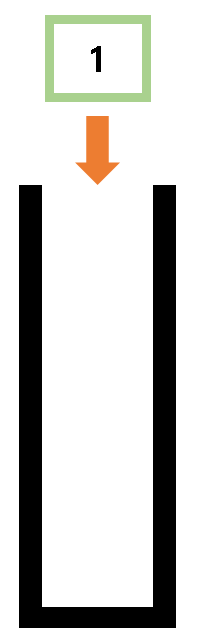
\includegraphics[]{stack2.png}\\
$1$이라는 값을 스택에 넣어줍시다.

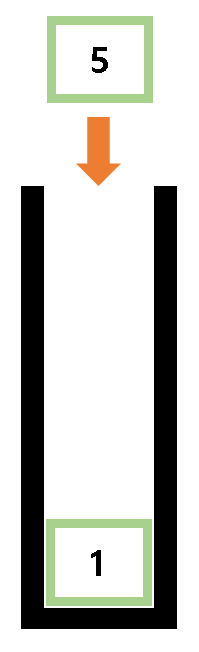
\includegraphics[]{stack3.png}\\
이 스택에 $5$이라는 값을 또 넣어줍시다.

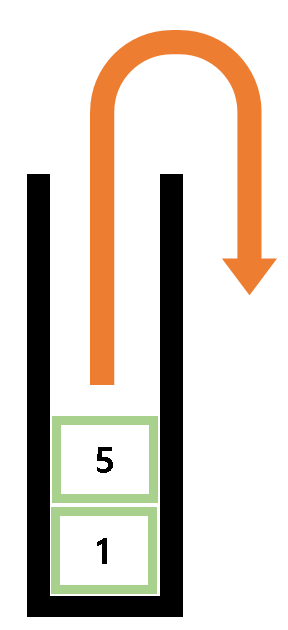
\includegraphics[]{stack4.png}\\
스택에서 맨 위의 값을 빼줍시다.\\
이때, 빠진 값은 스택에 먼저 넣은 $1$이 아닌, 나중에 넣은 $5$입니다. 스택은 Last in First Out, LIFO 구조로 나중에 넣은 값이 먼저 빠져나가게 됩니다.\\

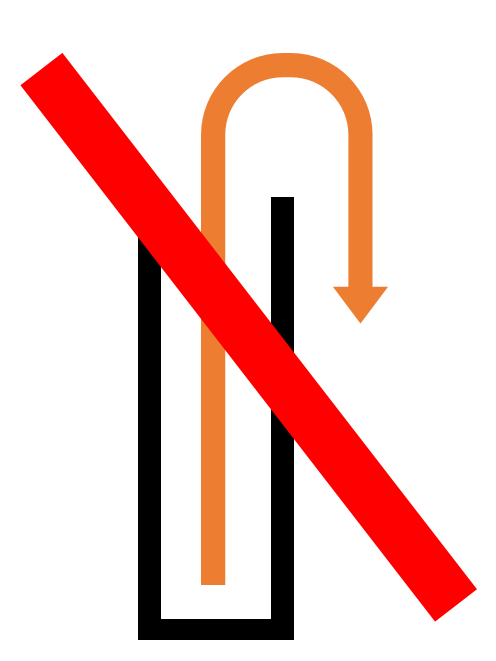
\includegraphics[]{stack5.png}\\
스택이 비어있는데 값을 빼려고 하면 문제가 발생합니다.\\\\

\noindent 그러면 스택이 어떤 것인지 대략적으로 감은 잡았는데, 아직 구체적으로 구현하기는 어려워 보입니다. 그림에서 values, tail의 2가지 변수를 생각해서 관리해봅시다. 각 변수의 역할은 아래와 같습니다.

\begin{itemize}
    \item values는 스택의 값들을 저장하는 공간입니다. 배열이나 벡터 등으로 구현할 수 있습니다.
    \item tail은 다음에 스택에 값을 넣을 때, 어디에 넣을지를 가리키는 변수입니다. 인덱스를 저장하는 변수로 사용하거나 포인터로 사용할 수 있습니다.
\end{itemize}

\noindent 스택에 값 x를 넣는 연산을 push(x), 스택 맨 위의 값을 빼고, 그 값을 반환하는 연산을 pop()연산으로 정의합시다. 이제 push(x) 연산은 values[tail++] = x로 수행할 수 있고, pop() 연산은 return values[--tail]을 통해 수행할 수 있습니다.\\\\

\noindent 시간복잡도\\\\
push(x) : $O(1)$\\
pop() : $O(1)$\\
top() : $O(1)$\\
size() : $O(1)$\\
isempty() : $O(1)$\\

\noindent 아래는 스택을 c++ class로 짠 코드입니다.\\

% code block
\lstset{style=myStyle}
\begin{lstlisting}[caption=소스코드, language=Matlab]
#include <iostream>
#include <assert.h>
using namespace std;

class Stack {
    private:
    int tail;
    int *values;
    int _size;

    public:
    void init(int initial_size) {
        tail = 0;
        _size = initial_size;
        values = new int[initial_size];
    }

    void push(int value) {
        assert(tail != _size); // Stack Overflow
        values[tail++] = value;
    }

    int pop() {
        assert(tail != 0); // Stack Underflow
        return values[--tail];
    }

    int top() {
        assert(tail != 0); // Stack is empty
        return values[tail - 1];
    }

    int __size() {
        return tail;
    }

    bool isEmpty() {
        return tail == 0;
    }

    bool isFull() {
        return tail == _size;
    }

    int* getValues() {
        return values;
    }
};

int main() {
    Stack* stack = new Stack();
    int initial_size;
    cout << "Enter initial stack size: ";
    cin >> initial_size;
    stack->init(initial_size);
    while (true) {
        int choice;
        cout << "1. Push\n2. Pop\n3. Top\n4. Size\n5. Is Empty\n6. Is Full\n7. Print Stack\n8. Exit\nEnter your choice: ";
        cin >> choice;
        if (choice == 1) {
            int value;
            cout << "Enter value to push: ";
            cin >> value;
            stack->push(value);
            cout << value << " pushed to stack\n";
        } else if (choice == 2) {
            cout << "Top element " << stack->pop() << " popped from stack\n";
        } else if (choice == 3) {
            cout << "Top element is " << stack->top() << "\n";
        } else if (choice == 4) {
            cout << "Stack size is " << stack->__size() << "\n";
        } else if (choice == 5) {
            cout << "Stack is " << (stack->isEmpty() ? "empty" : "not empty") << "\n";
        } else if (choice == 6) {
            cout << "Stack is " << (stack->isFull() ? "full" : "not full") << "\n";
        } else if (choice == 7) {
            int* vals = stack->getValues();
            cout << "Stack elements: ";
            for (int i = 0; i < stack->__size(); i++) {
                cout << vals[i] << " ";
            }
            cout << "\n";
        } else if (choice == 8) {
            break;
        } else {
            cout << "Invalid choice, please try again.\n";
        }
    }
    delete stack;
    return 0;
}
\end{lstlisting}

각 함수를 어떻게 구현할 수 있는지 살펴봅시다.
\begin{itemize}
    \item init()은 초기 스택의 최대 크기를 설정하고 tail = 0으로 설정하여 스택에 값을 넣고 뺄 수 있게 한 함수입니다.
    \item push(x)는 values[tail++] = x를 수행하여 스택에 값을 넣습니다. 이때, 스택에 할당한 메모리 이상에 접근하면 문제가 발생하므로 assert문으로 예외처리하여 줍시다.
    \item pop()은 return value[--tail]을 수행하여 스택의 가장 위 값을 return해주면서 stack의 크기를 1 줄여줍니다. 마찬가지로 tail == 0인 경우 음수 인덱스에 접근하여 문제가 발생하므로 assert문으로 예외처리하여 줍시다.
    \item top()은 return value[tail-1]을 수행하여 스택의 가장 위 값을 return해줍니다. pop()과 같이 tail == 0인 경우 음수 인덱스에 접근하여 문제가 발생하므로 assert문으로 예외처리하여 줍시다.
    \item \_\_size()는 스택의 크기를 반환합니다. 이때, 스택에는 0부터 tail-1까지의 인덱스에 값이 채워져 있고, 이때 크기는 tail이므로 return tail을 수행합니다.
    \item isEmpty()는 스택이 비어있는지 체크합니다. tail == 0이면 비어있는 것이고, 아니면 비어있지 않은 것이므로 return tail == 0을 수행합니다.
    \item isFull()은 스택의 크기와 할당된 메모리의 크기가 같은지 체크합니다. 초기에 할당한 메모리의 크기를 \_size에 저장하고 return tail == \_size를 수행합니다. tail == \_size이면 최대 크기이므로 이를 return하여 줍시다.
    \item getValues()는 스택 전체의 값을 출력하는 함수입니다. 원래는 존재하지도 않고, 스택의 연산에도 속하지 않지만, 스택의 값을 실시간으로 파악할 수 있도록 출력해주는 함수입니다.
\end{itemize}

\noindent 이제 어떻게 구현할 수 있는지까지 다 알아보았으니 문제를 풀어봅시다.\\\\
백준 10828번: 스택 \href{https://www.acmicpc.net/problem/10828}{https://www.acmicpc.net/problem/10828}\\\\

\noindent 그냥 위 템플릿과 유사하게 문제의 입출력 형식에 맞추어 스택의 연산을 수행해주면 문제를 해결할 수 있습니다. 이때, 스택의 메모리에 최대 10000개의 정수가 입력될 수 있으므로 최대 크기를 유의해서 잡아줍시다.\\\\

\noindent 소스코드\\
% code block
\lstset{style=myStyle}
\begin{lstlisting}[caption=소스코드, language=Matlab]
#include <iostream>
#include <assert.h>
using namespace std;

class Stack {
    private:
    int tail;
    int *values;
    int _size;

    public:
    void init(int initial_size) {
        tail = 0;
        _size = initial_size;
        values = new int[initial_size];
    }

    void push(int value) {
        assert(tail != _size); // Stack Overflow
        values[tail++] = value;
    }

    int pop() {
        assert(tail != 0); // Stack Underflow
        return values[--tail];
    }

    int top() {
        assert(tail != 0); // Stack is empty
        return values[tail - 1];
    }

    int __size() {
        return tail;
    }

    bool isEmpty() {
        return tail == 0;
    }

    bool isFull() {
        return tail == _size;
    }

    int* getValues() {
        return values;
    }
};

int main() {
    Stack* stack = new Stack();
    int initial_size;
    cin >> initial_size;
    stack->init(initial_size + 1);
    while (initial_size--) {
        string option;
        cin >> option;
        if (option == "push") {
            int value;
            cin >> value;
            stack->push(value);
        } else if (option == "pop") {
            if (stack->isEmpty())cout << -1 << "\n";
            else cout << stack->pop() << "\n";
        } else if (option == "top") {
            if (stack->isEmpty())cout << -1 << "\n";
            else cout << stack->top() << "\n";
        } else if (option == "size") {
            cout << stack->__size() << "\n";
        } else if (option == "empty") {
            cout << (stack->isEmpty() ? "1" : "0") << "\n";
        }
    }
    delete stack;
    return 0;
}
\end{lstlisting}

\noindent 꼭 매번 이렇게 코드를 길게 작성하여야 할까요? 그렇지는 않습니다. 코드를 구현하기 위한 간단한 구현체도 존재하고, 편리하게 사용하게 해주는 라이브러리도 존재합니다.\\

\noindent 보통 저는 아래처럼 class를 정의하지 않고 간단하게 구현하여 문제를 해결합니다.

\noindent 소스코드\\
% code block
\lstset{style=myStyle}
\begin{lstlisting}[caption=소스코드, language=Matlab]
#include <iostream>
#include <assert.h>
using namespace std;

int stack[10005],tail;

int main() {
    int t;
    scanf("%d",&t);
    while (t--) {
        string option;
        cin >> option;
        if (option == "push") {
            int v;
            cin >> v;
            stack[tail++] = v;
        } else if (option == "pop") {
            if (tail == 0)cout << -1 << "\n";
            else cout << stack[--tail] << "\n";
        } else if (option == "top") {
            if (tail == 0)cout << -1 << "\n";
            else cout << stack[tail-1] << "\n";
        } else if (option == "size") {
            cout << tail << "\n";
        } else if (option == "empty") {
            cout << (tail ? "0" : "1") << "\n";
        }
    }
    return 0;
}
\end{lstlisting}

\noindent 또, \<stack 라이브러리에 stack 구현체가 존재합니다. (deque를 안다면 실제로는 deque로 구현되어 있다는 것을 참고하면 좋습니다.)\\
해당 라이브러리에서도 구현해놓은 stack의 연산들을 사용할 수 있습니다.\\


\noindent 연습문제\\\\
백준 28278번: 스택 2 \href{https://www.acmicpc.net/problem/28278}{https://www.acmicpc.net/problem/28278}\\
백준 9012번: 괄호 \href{https://www.acmicpc.net/problem/9012}{https://www.acmicpc.net/problem/9012}\\
백준 1874번: 스택 수 \href{https://www.acmicpc.net/problem/1874}{https://www.acmicpc.net/problem/1874}\\
백준 2493번: 탑 \href{https://www.acmicpc.net/problem/2493}{https://www.acmicpc.net/problem/2493}\\
백준 6549번: 히스토그램에서 가장 큰 직사각형 \href{https://www.acmicpc.net/problem/6549}{https://www.acmicpc.net/problem/6549}\\
백준 11873번: 최대 직사각형 \href{https://www.acmicpc.net/problem/11873}{https://www.acmicpc.net/problem/11873}\\

\end{document}
